% Options for packages loaded elsewhere
\PassOptionsToPackage{unicode}{hyperref}
\PassOptionsToPackage{hyphens}{url}
%
\documentclass[
]{article}
\usepackage{amsmath,amssymb}
\usepackage{iftex}
\ifPDFTeX
  \usepackage[T1]{fontenc}
  \usepackage[utf8]{inputenc}
  \usepackage{textcomp} % provide euro and other symbols
\else % if luatex or xetex
  \usepackage{unicode-math} % this also loads fontspec
  \defaultfontfeatures{Scale=MatchLowercase}
  \defaultfontfeatures[\rmfamily]{Ligatures=TeX,Scale=1}
\fi
\usepackage{lmodern}
\ifPDFTeX\else
  % xetex/luatex font selection
\fi
% Use upquote if available, for straight quotes in verbatim environments
\IfFileExists{upquote.sty}{\usepackage{upquote}}{}
\IfFileExists{microtype.sty}{% use microtype if available
  \usepackage[]{microtype}
  \UseMicrotypeSet[protrusion]{basicmath} % disable protrusion for tt fonts
}{}
\makeatletter
\@ifundefined{KOMAClassName}{% if non-KOMA class
  \IfFileExists{parskip.sty}{%
    \usepackage{parskip}
  }{% else
    \setlength{\parindent}{0pt}
    \setlength{\parskip}{6pt plus 2pt minus 1pt}}
}{% if KOMA class
  \KOMAoptions{parskip=half}}
\makeatother
\usepackage{xcolor}
\usepackage[margin=1in]{geometry}
\usepackage{color}
\usepackage{fancyvrb}
\newcommand{\VerbBar}{|}
\newcommand{\VERB}{\Verb[commandchars=\\\{\}]}
\DefineVerbatimEnvironment{Highlighting}{Verbatim}{commandchars=\\\{\}}
% Add ',fontsize=\small' for more characters per line
\usepackage{framed}
\definecolor{shadecolor}{RGB}{248,248,248}
\newenvironment{Shaded}{\begin{snugshade}}{\end{snugshade}}
\newcommand{\AlertTok}[1]{\textcolor[rgb]{0.94,0.16,0.16}{#1}}
\newcommand{\AnnotationTok}[1]{\textcolor[rgb]{0.56,0.35,0.01}{\textbf{\textit{#1}}}}
\newcommand{\AttributeTok}[1]{\textcolor[rgb]{0.13,0.29,0.53}{#1}}
\newcommand{\BaseNTok}[1]{\textcolor[rgb]{0.00,0.00,0.81}{#1}}
\newcommand{\BuiltInTok}[1]{#1}
\newcommand{\CharTok}[1]{\textcolor[rgb]{0.31,0.60,0.02}{#1}}
\newcommand{\CommentTok}[1]{\textcolor[rgb]{0.56,0.35,0.01}{\textit{#1}}}
\newcommand{\CommentVarTok}[1]{\textcolor[rgb]{0.56,0.35,0.01}{\textbf{\textit{#1}}}}
\newcommand{\ConstantTok}[1]{\textcolor[rgb]{0.56,0.35,0.01}{#1}}
\newcommand{\ControlFlowTok}[1]{\textcolor[rgb]{0.13,0.29,0.53}{\textbf{#1}}}
\newcommand{\DataTypeTok}[1]{\textcolor[rgb]{0.13,0.29,0.53}{#1}}
\newcommand{\DecValTok}[1]{\textcolor[rgb]{0.00,0.00,0.81}{#1}}
\newcommand{\DocumentationTok}[1]{\textcolor[rgb]{0.56,0.35,0.01}{\textbf{\textit{#1}}}}
\newcommand{\ErrorTok}[1]{\textcolor[rgb]{0.64,0.00,0.00}{\textbf{#1}}}
\newcommand{\ExtensionTok}[1]{#1}
\newcommand{\FloatTok}[1]{\textcolor[rgb]{0.00,0.00,0.81}{#1}}
\newcommand{\FunctionTok}[1]{\textcolor[rgb]{0.13,0.29,0.53}{\textbf{#1}}}
\newcommand{\ImportTok}[1]{#1}
\newcommand{\InformationTok}[1]{\textcolor[rgb]{0.56,0.35,0.01}{\textbf{\textit{#1}}}}
\newcommand{\KeywordTok}[1]{\textcolor[rgb]{0.13,0.29,0.53}{\textbf{#1}}}
\newcommand{\NormalTok}[1]{#1}
\newcommand{\OperatorTok}[1]{\textcolor[rgb]{0.81,0.36,0.00}{\textbf{#1}}}
\newcommand{\OtherTok}[1]{\textcolor[rgb]{0.56,0.35,0.01}{#1}}
\newcommand{\PreprocessorTok}[1]{\textcolor[rgb]{0.56,0.35,0.01}{\textit{#1}}}
\newcommand{\RegionMarkerTok}[1]{#1}
\newcommand{\SpecialCharTok}[1]{\textcolor[rgb]{0.81,0.36,0.00}{\textbf{#1}}}
\newcommand{\SpecialStringTok}[1]{\textcolor[rgb]{0.31,0.60,0.02}{#1}}
\newcommand{\StringTok}[1]{\textcolor[rgb]{0.31,0.60,0.02}{#1}}
\newcommand{\VariableTok}[1]{\textcolor[rgb]{0.00,0.00,0.00}{#1}}
\newcommand{\VerbatimStringTok}[1]{\textcolor[rgb]{0.31,0.60,0.02}{#1}}
\newcommand{\WarningTok}[1]{\textcolor[rgb]{0.56,0.35,0.01}{\textbf{\textit{#1}}}}
\usepackage{graphicx}
\makeatletter
\def\maxwidth{\ifdim\Gin@nat@width>\linewidth\linewidth\else\Gin@nat@width\fi}
\def\maxheight{\ifdim\Gin@nat@height>\textheight\textheight\else\Gin@nat@height\fi}
\makeatother
% Scale images if necessary, so that they will not overflow the page
% margins by default, and it is still possible to overwrite the defaults
% using explicit options in \includegraphics[width, height, ...]{}
\setkeys{Gin}{width=\maxwidth,height=\maxheight,keepaspectratio}
% Set default figure placement to htbp
\makeatletter
\def\fps@figure{htbp}
\makeatother
\setlength{\emergencystretch}{3em} % prevent overfull lines
\providecommand{\tightlist}{%
  \setlength{\itemsep}{0pt}\setlength{\parskip}{0pt}}
\setcounter{secnumdepth}{-\maxdimen} % remove section numbering
\ifLuaTeX
  \usepackage{selnolig}  % disable illegal ligatures
\fi
\IfFileExists{bookmark.sty}{\usepackage{bookmark}}{\usepackage{hyperref}}
\IfFileExists{xurl.sty}{\usepackage{xurl}}{} % add URL line breaks if available
\urlstyle{same}
\hypersetup{
  pdftitle={Bellabeat Data Analysis Case Study},
  hidelinks,
  pdfcreator={LaTeX via pandoc}}

\title{Bellabeat Data Analysis Case Study}
\author{}
\date{\vspace{-2.5em}}

\begin{document}
\maketitle

\hypertarget{introduction}{%
\subsubsection{Introduction}\label{introduction}}

Bellabeat, founded by Urška Sršen and Sando Mur, is a high-tech company
that produces health-focused smart products for women. The aim of this
case study is to analyze smart device data to uncover insights into
consumer habits, which will inform Bellabeat's marketing strategy and
potentially unlock new growth opportunities.

\hypertarget{ask}{%
\section{Ask}\label{ask}}

\hypertarget{problem-statement}{%
\subsubsection{Problem Statement}\label{problem-statement}}

The primary objective is to analyze consumer usage data of non-Bellabeat
smart devices, focusing on identifying trends and applying these
insights to one of Bellabeat's products. The analysis will guide the
marketing strategy by answering the following questions:

\begin{itemize}
\tightlist
\item
  What are the trends in smart device usage?
\item
  How could these trends apply to Bellabeat customers?
\item
  How could these trends help influence Bellabeat marketing strategy?
\end{itemize}

\hypertarget{stakeholders}{%
\subsubsection{Stakeholders}\label{stakeholders}}

Primary stakeholders:

\begin{itemize}
\tightlist
\item
  Urška Sršen: Bellabeat's cofounder and Chief Creative Officer
\item
  Sando Mur: Mathematician and Bellabeat's cofounder
\end{itemize}

Secondary Stakeholders:

\begin{itemize}
\tightlist
\item
  Bellabeat marketing analytics team
\end{itemize}

\hypertarget{prepare}{%
\section{Prepare}\label{prepare}}

\hypertarget{data-source-and-location}{%
\paragraph{Data Source and Location}\label{data-source-and-location}}

Our foundational dataset is the FitBit Fitness Tracker Data, available
on \href{https://www.kaggle.com/datasets/arashnic/fitbit}{Kaggle}. This
dataset, generated by 30 Fitbit users, spans from 03.12.2016 to
05.12.2016, offering insights into daily activities, physical activity,
heart rate, and sleep patterns.

\hypertarget{acknowledgement-and-licensing}{%
\paragraph{Acknowledgement and
Licensing}\label{acknowledgement-and-licensing}}

The dataset, created by Furberg, Robert; Brinton, Julia; Keating,
Michael; and Ortiz, Alexa, is documented on
\href{https://zenodo.org/record/53894\#.YMoUpnVKiP9}{Zenodo} and
licensed under CC0: Public Domain.

\hypertarget{data-organization-and-integrity}{%
\paragraph{Data Organization and
Integrity}\label{data-organization-and-integrity}}

Organized in 18 CSV files, each focusing on different aspects of user
activity, the dataset has been scrutinized for errors and
inconsistencies to ensure its integrity and reliability.

\hypertarget{process}{%
\section{Process}\label{process}}

\hypertarget{tools-and-data-cleaning}{%
\subsubsection{Tools and Data Cleaning}\label{tools-and-data-cleaning}}

R is chosen as the primary tool for its extensive libraries and
capabilities in handling, analyzing, and visualizing data. The data
cleaning process involves formatting timestamps, merging data frames,
and handling missing or erroneous data to ensure integrity.

\hypertarget{r-code-for-data-loading}{%
\subsubsection{R Code for Data Loading}\label{r-code-for-data-loading}}

\begin{Shaded}
\begin{Highlighting}[]
\CommentTok{\# Load necessary libraries}
\FunctionTok{library}\NormalTok{(tidyverse)}
\end{Highlighting}
\end{Shaded}

\begin{verbatim}
## -- Attaching core tidyverse packages ------------------------ tidyverse 2.0.0 --
## v dplyr     1.1.2     v readr     2.1.4
## v forcats   1.0.0     v stringr   1.5.0
## v ggplot2   3.4.3     v tibble    3.2.1
## v lubridate 1.9.2     v tidyr     1.3.0
## v purrr     1.0.2     
## -- Conflicts ------------------------------------------ tidyverse_conflicts() --
## x dplyr::filter() masks stats::filter()
## x dplyr::lag()    masks stats::lag()
## i Use the conflicted package (<http://conflicted.r-lib.org/>) to force all conflicts to become errors
\end{verbatim}

\begin{Shaded}
\begin{Highlighting}[]
\FunctionTok{library}\NormalTok{(lubridate)}

\CommentTok{\# Define the common path prefix}
\NormalTok{path\_prefix }\OtherTok{\textless{}{-}} \StringTok{"C:/Users/jorda/OneDrive/Documents/Coursera/Capstone/Fitabase Data 4.12.16{-}5.12.16/"}

\CommentTok{\# Check if files exist before loading}
\NormalTok{files }\OtherTok{\textless{}{-}} \FunctionTok{c}\NormalTok{(}\StringTok{"dailyActivity\_merged.csv"}\NormalTok{, }\StringTok{"hourlyCalories\_merged.csv"}\NormalTok{, }
           \StringTok{"hourlyIntensities\_merged.csv"}\NormalTok{, }\StringTok{"sleepDay\_merged.csv"}\NormalTok{, }
           \StringTok{"weightLogInfo\_merged.csv"}\NormalTok{)}
\ControlFlowTok{for}\NormalTok{ (file }\ControlFlowTok{in}\NormalTok{ files) \{}
  \ControlFlowTok{if}\NormalTok{ (}\SpecialCharTok{!}\FunctionTok{file.exists}\NormalTok{(}\FunctionTok{paste0}\NormalTok{(path\_prefix, file))) \{}
    \FunctionTok{stop}\NormalTok{(}\FunctionTok{paste0}\NormalTok{(}\StringTok{"File not found: "}\NormalTok{, path\_prefix, file))}
\NormalTok{  \}}
\NormalTok{\}}

\CommentTok{\# Load the data}
\NormalTok{activity }\OtherTok{\textless{}{-}} \FunctionTok{read.csv}\NormalTok{(}\FunctionTok{paste0}\NormalTok{(path\_prefix, }\StringTok{"dailyActivity\_merged.csv"}\NormalTok{))}
\NormalTok{calories }\OtherTok{\textless{}{-}} \FunctionTok{read.csv}\NormalTok{(}\FunctionTok{paste0}\NormalTok{(path\_prefix, }\StringTok{"hourlyCalories\_merged.csv"}\NormalTok{))}
\NormalTok{intensities }\OtherTok{\textless{}{-}} \FunctionTok{read.csv}\NormalTok{(}\FunctionTok{paste0}\NormalTok{(path\_prefix, }\StringTok{"hourlyIntensities\_merged.csv"}\NormalTok{))}
\NormalTok{sleep }\OtherTok{\textless{}{-}} \FunctionTok{read.csv}\NormalTok{(}\FunctionTok{paste0}\NormalTok{(path\_prefix, }\StringTok{"sleepDay\_merged.csv"}\NormalTok{))}
\NormalTok{weight }\OtherTok{\textless{}{-}} \FunctionTok{read.csv}\NormalTok{(}\FunctionTok{paste0}\NormalTok{(path\_prefix, }\StringTok{"weightLogInfo\_merged.csv"}\NormalTok{))}
\end{Highlighting}
\end{Shaded}

\hypertarget{data-cleaning-and-formatting}{%
\subsubsection{Data Cleaning and
Formatting}\label{data-cleaning-and-formatting}}

\begin{Shaded}
\begin{Highlighting}[]
\CommentTok{\# Format timestamp columns}
\NormalTok{format\_timestamp }\OtherTok{\textless{}{-}} \ControlFlowTok{function}\NormalTok{(data, timestamp\_col) \{}
\NormalTok{  data[[timestamp\_col]] }\OtherTok{\textless{}{-}} \FunctionTok{as.POSIXct}\NormalTok{(data[[timestamp\_col]], }\AttributeTok{format=}\StringTok{"\%m/\%d/\%Y \%I:\%M:\%S \%p"}\NormalTok{, }\AttributeTok{tz=}\StringTok{"UTC"}\NormalTok{)}
\NormalTok{  data}\SpecialCharTok{$}\NormalTok{date }\OtherTok{\textless{}{-}} \FunctionTok{format}\NormalTok{(data[[timestamp\_col]], }\AttributeTok{format=}\StringTok{"\%Y{-}\%m{-}\%d"}\NormalTok{)}
\NormalTok{  data}\SpecialCharTok{$}\NormalTok{time }\OtherTok{\textless{}{-}} \FunctionTok{format}\NormalTok{(data[[timestamp\_col]], }\AttributeTok{format=}\StringTok{"\%H:\%M:\%S"}\NormalTok{)}
  \FunctionTok{return}\NormalTok{(data)}
\NormalTok{\}}

\CommentTok{\# Apply the formatting function to relevant columns}
\NormalTok{intensities }\OtherTok{\textless{}{-}} \FunctionTok{format\_timestamp}\NormalTok{(intensities, }\StringTok{"ActivityHour"}\NormalTok{)}
\NormalTok{calories }\OtherTok{\textless{}{-}} \FunctionTok{format\_timestamp}\NormalTok{(calories, }\StringTok{"ActivityHour"}\NormalTok{)}
\NormalTok{activity}\SpecialCharTok{$}\NormalTok{date }\OtherTok{\textless{}{-}} \FunctionTok{as.Date}\NormalTok{(activity}\SpecialCharTok{$}\NormalTok{ActivityDate, }\AttributeTok{format=}\StringTok{"\%m/\%d/\%Y"}\NormalTok{)}
\NormalTok{sleep }\OtherTok{\textless{}{-}} \FunctionTok{format\_timestamp}\NormalTok{(sleep, }\StringTok{"SleepDay"}\NormalTok{)}

\CommentTok{\# Merge the data frames using \textquotesingle{}Id\textquotesingle{} and \textquotesingle{}date\textquotesingle{} columns}
\NormalTok{merged\_data }\OtherTok{\textless{}{-}} \FunctionTok{merge}\NormalTok{(activity, sleep, }\AttributeTok{by=}\FunctionTok{c}\NormalTok{(}\StringTok{\textquotesingle{}Id\textquotesingle{}}\NormalTok{, }\StringTok{\textquotesingle{}date\textquotesingle{}}\NormalTok{))}
\end{Highlighting}
\end{Shaded}

\hypertarget{analyze}{%
\section{Analyze}\label{analyze}}

\hypertarget{exploratory-data-analysis-eda}{%
\subsubsection{Exploratory Data Analysis
(EDA)}\label{exploratory-data-analysis-eda}}

The analysis involves calculating summary statistics, performing
correlation tests, and exploring relationships between different
variables to identify patterns and trends in smart device usage.

\begin{Shaded}
\begin{Highlighting}[]
\CommentTok{\# Calculate summary statistics for various variables}
\NormalTok{variables }\OtherTok{\textless{}{-}} \FunctionTok{c}\NormalTok{(}\StringTok{"TotalSteps"}\NormalTok{, }\StringTok{"Calories"}\NormalTok{, }\StringTok{"TotalMinutesAsleep"}\NormalTok{, }\StringTok{"TotalTimeInBed"}\NormalTok{)}
\ControlFlowTok{for}\NormalTok{ (var }\ControlFlowTok{in}\NormalTok{ variables) \{}
  \FunctionTok{print}\NormalTok{(}\FunctionTok{paste0}\NormalTok{(}\StringTok{"Summary Statistics for "}\NormalTok{, var, }\StringTok{":"}\NormalTok{))}
  \FunctionTok{print}\NormalTok{(}\FunctionTok{summary}\NormalTok{(merged\_data[[var]]))}
\NormalTok{\}}
\end{Highlighting}
\end{Shaded}

\begin{verbatim}
## [1] "Summary Statistics for TotalSteps:"
##    Min. 1st Qu.  Median    Mean 3rd Qu.    Max. 
##      17    5206    8925    8541   11393   22770 
## [1] "Summary Statistics for Calories:"
##    Min. 1st Qu.  Median    Mean 3rd Qu.    Max. 
##     257    1850    2220    2398    2926    4900 
## [1] "Summary Statistics for TotalMinutesAsleep:"
##    Min. 1st Qu.  Median    Mean 3rd Qu.    Max. 
##    58.0   361.0   433.0   419.5   490.0   796.0 
## [1] "Summary Statistics for TotalTimeInBed:"
##    Min. 1st Qu.  Median    Mean 3rd Qu.    Max. 
##    61.0   403.0   463.0   458.6   526.0   961.0
\end{verbatim}

\begin{Shaded}
\begin{Highlighting}[]
\CommentTok{\# Perform a correlation test between Total Steps and Calories Burned}
\NormalTok{cor\_test }\OtherTok{\textless{}{-}} \FunctionTok{cor.test}\NormalTok{(activity}\SpecialCharTok{$}\NormalTok{TotalSteps, activity}\SpecialCharTok{$}\NormalTok{Calories)}
\FunctionTok{print}\NormalTok{(}\StringTok{"Correlation Test between Total Steps and Calories Burned:"}\NormalTok{)}
\end{Highlighting}
\end{Shaded}

\begin{verbatim}
## [1] "Correlation Test between Total Steps and Calories Burned:"
\end{verbatim}

\begin{Shaded}
\begin{Highlighting}[]
\FunctionTok{print}\NormalTok{(cor\_test)}
\end{Highlighting}
\end{Shaded}

\begin{verbatim}
## 
##  Pearson's product-moment correlation
## 
## data:  activity$TotalSteps and activity$Calories
## t = 22.472, df = 938, p-value < 2.2e-16
## alternative hypothesis: true correlation is not equal to 0
## 95 percent confidence interval:
##  0.5483688 0.6316184
## sample estimates:
##       cor 
## 0.5915681
\end{verbatim}

\hypertarget{interpretation-of-results}{%
\subsubsection{Interpretation of
Results}\label{interpretation-of-results}}

\begin{itemize}
\tightlist
\item
  There is a significant positive correlation between Total Steps and
  Calories Burned (correlation coefficient: 0.59, p-value \textless{}
  2.2e-16). This implies that as the number of steps increases, the
  number of calories burned also increases.
\item
  Summary statistics for variables like TotalSteps, Calories, and
  TotalMinutesAsleep show varying ranges, indicating diversity in user
  behavior.
\end{itemize}

\hypertarget{share}{%
\section{Share}\label{share}}

\hypertarget{visualization}{%
\subsubsection{Visualization}\label{visualization}}

\begin{Shaded}
\begin{Highlighting}[]
\CommentTok{\# Total Steps vs. Calories Burned with Hexbin Plot and Regression Line}
\FunctionTok{ggplot}\NormalTok{(}\AttributeTok{data=}\NormalTok{activity, }\FunctionTok{aes}\NormalTok{(}\AttributeTok{x=}\NormalTok{TotalSteps, }\AttributeTok{y=}\NormalTok{Calories)) }\SpecialCharTok{+} 
  \FunctionTok{geom\_hex}\NormalTok{(}\AttributeTok{bins=}\DecValTok{50}\NormalTok{, }\AttributeTok{color=}\StringTok{"white"}\NormalTok{) }\SpecialCharTok{+} 
  \FunctionTok{geom\_smooth}\NormalTok{(}\AttributeTok{method=}\StringTok{"lm"}\NormalTok{, }\AttributeTok{se=}\ConstantTok{FALSE}\NormalTok{, }\AttributeTok{color=}\StringTok{"red"}\NormalTok{) }\SpecialCharTok{+}
  \FunctionTok{labs}\NormalTok{(}\AttributeTok{title=}\StringTok{"Total Steps vs. Calories Burned"}\NormalTok{, }\AttributeTok{x=}\StringTok{"Total Steps"}\NormalTok{, }\AttributeTok{y=}\StringTok{"Calories Burned"}\NormalTok{) }\SpecialCharTok{+}
  \FunctionTok{theme\_minimal}\NormalTok{()}
\end{Highlighting}
\end{Shaded}

\begin{verbatim}
## `geom_smooth()` using formula = 'y ~ x'
\end{verbatim}

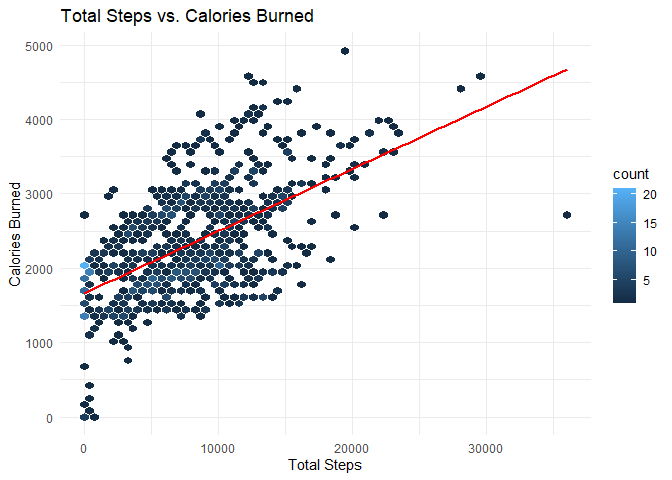
\includegraphics{bellabeat_case_study_files/figure-latex/unnamed-chunk-4-1.pdf}

\begin{Shaded}
\begin{Highlighting}[]
\CommentTok{\# Sleep Duration vs. Total Steps (Activity Level) with Jitter and Regression Line}
\FunctionTok{ggplot}\NormalTok{(}\AttributeTok{data=}\NormalTok{merged\_data, }\FunctionTok{aes}\NormalTok{(}\AttributeTok{x=}\NormalTok{TotalMinutesAsleep, }\AttributeTok{y=}\NormalTok{TotalSteps)) }\SpecialCharTok{+} 
  \FunctionTok{geom\_jitter}\NormalTok{(}\AttributeTok{shape=}\DecValTok{1}\NormalTok{, }\AttributeTok{color=}\StringTok{"darkblue"}\NormalTok{, }\AttributeTok{width=}\FloatTok{0.3}\NormalTok{, }\AttributeTok{height=}\FloatTok{0.3}\NormalTok{) }\SpecialCharTok{+}
  \FunctionTok{geom\_smooth}\NormalTok{(}\AttributeTok{method=}\StringTok{"lm"}\NormalTok{, }\AttributeTok{se=}\ConstantTok{FALSE}\NormalTok{, }\AttributeTok{color=}\StringTok{"red"}\NormalTok{) }\SpecialCharTok{+}
  \FunctionTok{labs}\NormalTok{(}\AttributeTok{title=}\StringTok{"Sleep Duration vs. Total Steps"}\NormalTok{, }\AttributeTok{x=}\StringTok{"Total Minutes Asleep"}\NormalTok{, }\AttributeTok{y=}\StringTok{"Total Steps (Activity Level)"}\NormalTok{) }\SpecialCharTok{+}
  \FunctionTok{theme\_minimal}\NormalTok{()}
\end{Highlighting}
\end{Shaded}

\begin{verbatim}
## `geom_smooth()` using formula = 'y ~ x'
\end{verbatim}

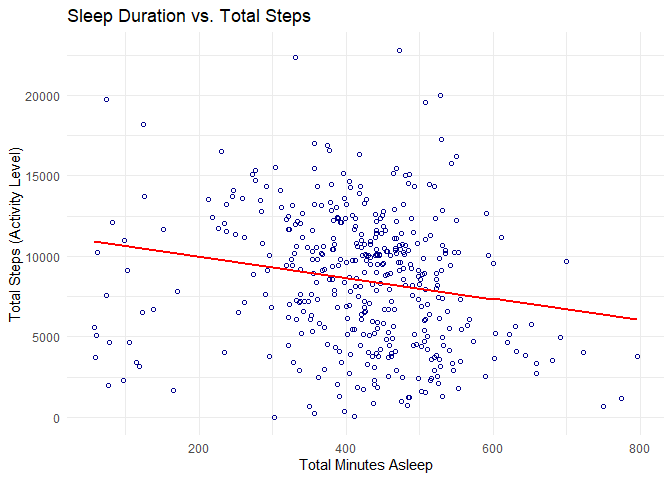
\includegraphics{bellabeat_case_study_files/figure-latex/unnamed-chunk-4-2.pdf}

\begin{Shaded}
\begin{Highlighting}[]
\CommentTok{\# Define Activity Level based on Total Steps}
\NormalTok{merged\_data}\SpecialCharTok{$}\NormalTok{ActivityLevel }\OtherTok{\textless{}{-}} \FunctionTok{cut}\NormalTok{(merged\_data}\SpecialCharTok{$}\NormalTok{TotalSteps, }
                                 \AttributeTok{breaks =} \FunctionTok{c}\NormalTok{(}\SpecialCharTok{{-}}\ConstantTok{Inf}\NormalTok{, }\DecValTok{5000}\NormalTok{, }\DecValTok{10000}\NormalTok{, }\ConstantTok{Inf}\NormalTok{), }
                                 \AttributeTok{labels =} \FunctionTok{c}\NormalTok{(}\StringTok{"Low"}\NormalTok{, }\StringTok{"Medium"}\NormalTok{, }\StringTok{"High"}\NormalTok{))}

\CommentTok{\# Sleep Duration vs. Activity Level with Box Plot}
\FunctionTok{ggplot}\NormalTok{(}\AttributeTok{data=}\NormalTok{merged\_data, }\FunctionTok{aes}\NormalTok{(}\AttributeTok{x=}\NormalTok{ActivityLevel, }\AttributeTok{y=}\NormalTok{TotalMinutesAsleep, }\AttributeTok{fill=}\NormalTok{ActivityLevel)) }\SpecialCharTok{+} 
  \FunctionTok{geom\_boxplot}\NormalTok{() }\SpecialCharTok{+}
  \FunctionTok{labs}\NormalTok{(}\AttributeTok{title=}\StringTok{"Sleep Duration vs. Activity Level"}\NormalTok{, }\AttributeTok{x=}\StringTok{"Activity Level"}\NormalTok{, }\AttributeTok{y=}\StringTok{"Total Minutes Asleep"}\NormalTok{) }\SpecialCharTok{+}
  \FunctionTok{theme\_minimal}\NormalTok{() }\SpecialCharTok{+}
  \FunctionTok{scale\_fill\_manual}\NormalTok{(}\AttributeTok{values=}\FunctionTok{c}\NormalTok{(}\StringTok{"Low"} \OtherTok{=} \StringTok{"lightblue"}\NormalTok{, }\StringTok{"Medium"} \OtherTok{=} \StringTok{"lightgreen"}\NormalTok{, }\StringTok{"High"} \OtherTok{=} \StringTok{"lightcoral"}\NormalTok{))}
\end{Highlighting}
\end{Shaded}

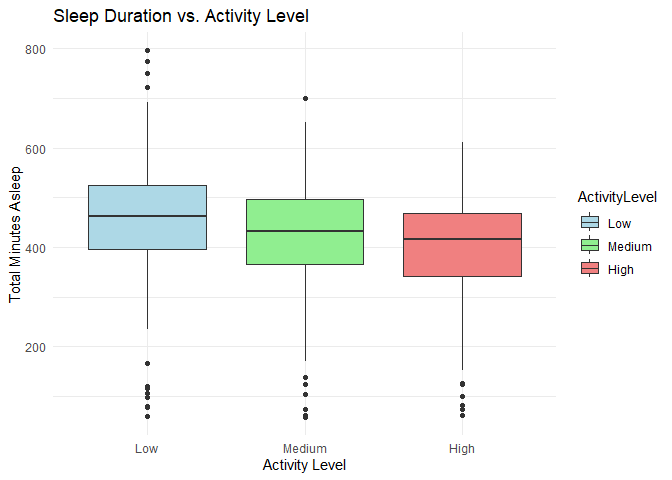
\includegraphics{bellabeat_case_study_files/figure-latex/unnamed-chunk-4-3.pdf}

\begin{Shaded}
\begin{Highlighting}[]
\CommentTok{\# Average Intensity Levels vs. Time with Line Plot and Shading}
\NormalTok{intensity\_avg }\OtherTok{\textless{}{-}}\NormalTok{ intensities }\SpecialCharTok{\%\textgreater{}\%}
  \FunctionTok{group\_by}\NormalTok{(time) }\SpecialCharTok{\%\textgreater{}\%}
  \FunctionTok{summarise}\NormalTok{(}\AttributeTok{avg\_intensity =} \FunctionTok{mean}\NormalTok{(TotalIntensity), }\AttributeTok{se =} \FunctionTok{sd}\NormalTok{(TotalIntensity) }\SpecialCharTok{/} \FunctionTok{sqrt}\NormalTok{(}\FunctionTok{n}\NormalTok{()))}

\CommentTok{\# Convert \textquotesingle{}time\textquotesingle{} to factor while keeping only the hour part for plotting}
\NormalTok{intensity\_avg}\SpecialCharTok{$}\NormalTok{time }\OtherTok{\textless{}{-}} \FunctionTok{factor}\NormalTok{(}\FunctionTok{format}\NormalTok{(}\FunctionTok{strptime}\NormalTok{(intensity\_avg}\SpecialCharTok{$}\NormalTok{time, }\AttributeTok{format=}\StringTok{"\%H:\%M:\%S"}\NormalTok{), }\StringTok{"\%H"}\NormalTok{), }\AttributeTok{levels =} \FunctionTok{sprintf}\NormalTok{(}\StringTok{"\%02d"}\NormalTok{, }\DecValTok{0}\SpecialCharTok{:}\DecValTok{23}\NormalTok{))}

\CommentTok{\# Create the line plot}
\FunctionTok{ggplot}\NormalTok{(}\AttributeTok{data=}\NormalTok{intensity\_avg, }\FunctionTok{aes}\NormalTok{(}\AttributeTok{x=}\NormalTok{time, }\AttributeTok{y=}\NormalTok{avg\_intensity)) }\SpecialCharTok{+} 
  \FunctionTok{geom\_line}\NormalTok{(}\AttributeTok{group=}\DecValTok{1}\NormalTok{, }\AttributeTok{color=}\StringTok{\textquotesingle{}darkblue\textquotesingle{}}\NormalTok{) }\SpecialCharTok{+}
  \FunctionTok{geom\_ribbon}\NormalTok{(}\FunctionTok{aes}\NormalTok{(}\AttributeTok{ymin=}\NormalTok{avg\_intensity}\SpecialCharTok{{-}}\NormalTok{se, }\AttributeTok{ymax=}\NormalTok{avg\_intensity}\SpecialCharTok{+}\NormalTok{se), }\AttributeTok{alpha=}\FloatTok{0.2}\NormalTok{) }\SpecialCharTok{+}
  \FunctionTok{scale\_x\_discrete}\NormalTok{(}\AttributeTok{breaks=}\FunctionTok{sprintf}\NormalTok{(}\StringTok{"\%02d"}\NormalTok{, }\DecValTok{0}\SpecialCharTok{:}\DecValTok{23}\NormalTok{)) }\SpecialCharTok{+}
  \FunctionTok{theme}\NormalTok{(}\AttributeTok{axis.text.x =} \FunctionTok{element\_text}\NormalTok{(}\AttributeTok{angle=}\DecValTok{45}\NormalTok{, }\AttributeTok{vjust=}\FloatTok{0.5}\NormalTok{, }\AttributeTok{hjust=}\DecValTok{1}\NormalTok{)) }\SpecialCharTok{+}
  \FunctionTok{labs}\NormalTok{(}\AttributeTok{title=}\StringTok{"Average Intensity Levels vs. Time"}\NormalTok{, }\AttributeTok{x=}\StringTok{"Time (Hour)"}\NormalTok{, }\AttributeTok{y=}\StringTok{"Average Intensity"}\NormalTok{) }\SpecialCharTok{+}
  \FunctionTok{theme\_minimal}\NormalTok{()}
\end{Highlighting}
\end{Shaded}

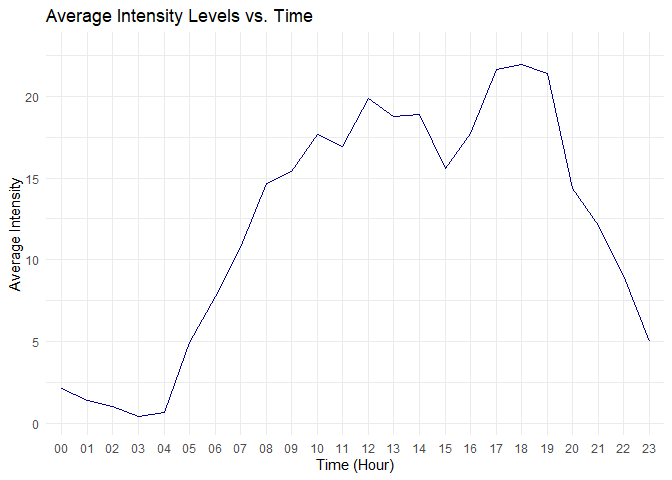
\includegraphics{bellabeat_case_study_files/figure-latex/unnamed-chunk-4-4.pdf}
\#\#\# Interpretation of Visualizations

\begin{itemize}
\tightlist
\item
  The Hexbin Plot shows a clear positive linear relationship between
  Total Steps and Calories Burned.
\item
  The scatter plot comparing Sleep Duration vs.~Total Steps shows a
  trend where individuals with higher sleep durations tend to have lower
  total steps.
\item
  The Box plot reveals variations in sleep duration across different
  activity levels, suggesting that individuals with higher activity
  levels tend to have shorter sleep durations.
\item
  The line plot comparing Average Intensity Levels vs.~Time shows that
  intensity peaks during morning and evening, suggesting popular times
  for workouts.
\end{itemize}

\hypertarget{act}{%
\section{Act}\label{act}}

\hypertarget{conclusions-and-recommendations}{%
\subsubsection{Conclusions and
Recommendations}\label{conclusions-and-recommendations}}

\begin{itemize}
\item
  \textbf{Targeted Marketing Campaigns}: Develop marketing campaigns
  targeting users with varying activity levels and sleep patterns,
  emphasizing how Bellabeat products can help achieve a balance between
  activity and rest.
\item
  \textbf{Personalized Health Goals}: Introduce features in Bellabeat
  app to set personalized daily step goals and sleep targets,
  encouraging users to maintain an active lifestyle while ensuring
  adequate rest.
\item
  \textbf{Sleep and Activity Insights}: Enhance the Bellabeat app with
  insights on the correlation between sleep duration and physical
  activity, educating users on the importance of balancing both for
  overall well-being.
\item
  \textbf{Peak Activity Notifications}: Send notifications during peak
  activity times to encourage workouts.
\item
  \textbf{Wellness Challenges and Rewards}: Launch wellness challenges
  focusing on achieving step goals and maintaining healthy sleep
  patterns, with rewards to keep users engaged and motivated.
\item
  \textbf{Educational Content}: Provide educational content and tips
  within the app on the benefits of regular physical activity and good
  sleep hygiene, helping users make informed lifestyle choices.
\item
  \textbf{User Segmentation for Communication}: Utilize data on user
  behavior to segment users based on their activity levels and sleep
  durations for targeted communication and personalized recommendations.
\end{itemize}

A larger sample size is needed for a more accurate analysis. These
recommendations aim to leverage the insights gained from the data
analysis to enhance user engagement, promote healthy lifestyles, and
drive growth for Bellabeat.

\end{document}
